\documentclass{report}
\usepackage[T1]{fontenc} % Fontes T1
\usepackage[utf8]{inputenc} % Input UTF8
\usepackage[backend=biber, style=ieee]{biblatex} % para usar bibliografia
\usepackage{csquotes}
\usepackage[portuguese]{babel} %Usar língua portuguesa
\usepackage{blindtext} % Gerar texto automaticamente
\usepackage[printonlyused]{acronym}
\usepackage{hyperref} % para autoref
\usepackage{graphicx}
\usepackage{indentfirst}
\bibliography{bibliografia}
\usepackage{csquotes}
\usepackage{blindtext} 
\usepackage[backend=biber, style=ieee]{biblatex}

\begin{document}
%%
% Definições
%
\def\titulo{CRISPR/Cas9}
\def\data{19 de dezembro de 2020}
\def\autores{Alexandre Costa Martins }
\def\autorescontactos{(103552) alexandremartins@ua.pt}
\def\versao{VERSAO 1}
\def\departamento{DETI - Universidade de Aveiro}
\def\empresa{Universidade de Aveiro}
\def\logotipo{ua.pdf}
%
%%%%%% CAPA %%%%%%
%

\renewcommand{\contentsname}{Índice}
\begin{titlepage}

\begin{center}
%
\vspace*{0mm}
%
{\Huge \titulo}\\ 
%
\vspace{50mm}
%
{\Large \empresa}\\
%
\vspace{10mm}
%
{\LARGE \autores}\\ 
%
\vspace{30mm}
%
\begin{figure}[h]
\center

\includegraphics{\logotipo}
\end{figure}
%
\vspace{30mm}
\end{center}
%
\begin{flushright}
\versao
\end{flushright}
\end{titlepage}

%%  Página de Título %%
\title{%
{\Huge\textbf{\titulo}}\\
{\Large \departamento}
}
%
\author{%
    \autores \\
    \autorescontactos
}
%
\date{\data}
%
\maketitle

\pagenumbering{roman}

%%%%%% RESUMO %%%%%%
\begin{abstract}
Uma das maiores e mais importantes histórias científicas dos últimos anos provavelmente também será uma das maiores histórias científicas dos próximos anos. 

Nos últimos nove anos, os cientistas descobriram como explorar uma peculiaridade do sistema imunológico das bactérias para editar genes em outros organismos - plantas, ratos, até mesmo humanos. Com o CRISPR, eles agora podem fazer essas edições de forma rápida e econômica, em dias em vez de semanas ou meses. (A tecnologia é frequentemente conhecida como CRISPR / Cas9, mas vamos ficar com \ac{crispr}, pronunciado "mais nítido".)\par
Esta é uma nova ferramenta com a capacidade de excluir características indesejáveis e, potencialmente, adicionar características desejáveis com mais precisão do que nunca.\par
Até agora, os cientistas usaram-no para reduzir a gravidade da surdez genética em ratos, sugerindo que um dia poderia ser usado para tratar o mesmo tipo de perda auditiva em pessoas. Eles criaram cogumelos que não escurecem facilmente e editaram células da medula óssea em joga para tratar a anemia falciforme. No futuro, o CRISPR pode nos ajudar a desenvolver safras tolerantes à seca e a criar novos antibióticos poderosos. O CRISPR poderia um dia até nos permitir exterminar populações inteiras de mosquitos transmissores da malária ou ressuscitar espécies outrora extintas, como o pombo-passageiro.

\end{abstract}

%%%%%% Agradecimentos %%%%%%
% Segundo glisc deveria aparecer após conclusão...
\renewcommand{\abstractname}{Agradecimentos}
\begin{abstract}
Queria agradecer a um familiar, Carlos Martins, por me ter proposto este tema de relatorio, pois com ele aprendi varias coisas que anteriormente não tinha noção como, por exemplo, as diferentes vantagens da utilização do CRISPR/Cas9 em produtos alimentares e na cura de doenças hereditarias.

\end{abstract}


\tableofcontents
% \listoftables     % descomentar se necessário
% \listoffigures    % descomentar se necessário


%%%%%%%%%%%%%%%%%%%%%%%%%%%%%%%
\clearpage
\pagenumbering{arabic}

%%%%%%%%%%%%%%%%%%%%%%%%%%%%%%%%
\chapter{Introdução}
\label{chap.introducao}

Neste relatório será abordado o tema "\ac{crispr}/Cas9", o qual pode vir a ser o próximo grande salto na conservação ou melhoraria do meio ambiente desde a indústria agrícola até setores da saúde humana. Este tema surgiu interesse pelo facto de pertencer a área que procuro seguir no futuro, Bioinformática.

Irá se tentar perceber no que consite a ferramenta de edição de genoma \ac{crispr}/Cas9, como funciona, as suas virtudes e limitações. Também será mencionanda a sua história e aplicações.

Este documento está dividido em cinco capitulos \par

Depois desta introdução,
no \autoref{chap.classificação} são apresentadas as duas classes existentes no sistema \ac{crispr} de seguida,
no \autoref{chap.anti-CRISPRs} são apresentados os Anti-CRISPRs,
seguem-se as diferentes aplicações de \ac{crispr}/Cas9 no \autoref{chap.aplicação}.
Finalmente, no \autoref{chap.conclusões} são apresentadas
as conclusões do trabalho.)
\begin{figure}[h]
\center
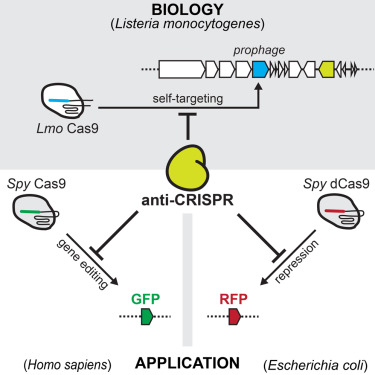
\includegraphics[scale=0.8]{pog}
\label{pog}
\caption{Listeria monocytogenes}
\end{figure}

\chapter{Classificação}
\label{chap.classificação}



Os sistemas \ac{crispr} – Cas fornecem imunidade adaptativa em arquéias e bactérias. As características e mecanismos estruturais do \ac{crispr}-Cas são descritos em detalhes em várias revisões recentes. Em resumo, a resposta \ac{crispr}-Cas consiste em três estágios. Durante o primeiro estágio, conhecido como adaptação, o complexo de proteína Cas1-Cas2 (que, em alguns casos, contém subunidades adicionais) retira um segmento do DNA alvo (conhecido como protoespaçador) e o insere entre as repetições na extremidade 5 ' de uma matriz \ac{crispr}, produzindo um novo espaçador. No estágio de expressão e processamento, uma matriz \ac{crispr}, juntamente com os espaçadores, é transcrita em um transcrito longo conhecido como RNA pré-\ac{crispr} (pré-crRNA) e é processada por um complexo distinto (que, em alguns casos , envolve proteínas adicionais e moléculas de RNA) de proteínas Cas em pequenos RNAs \ac{crispr} maduros (crRNAs). Finalmente, durante o estágio de interferência, um complexo de proteínas Cas (tipicamente, um complexo de processamento modificado) usa o crRNA como um guia para clivar o DNA ou RNA alvo. Da mesma forma que outros mecanismos de defesa, os sistemas \ac{crispr}-Cas evoluíram no contexto de uma incessante corrida armamentista com elementos genéticos móveis, o que resultou em extrema diversificação das sequências da proteína Cas e na arquitetura dos loci \ac{crispr}-cas7-12. Devido a esta diversidade e à falta de genes cas universais, uma classificação abrangente de sistemas \ac{crispr}-Cas não pode ser gerada como uma única árvore filogenética, mas requer uma abordagem multifacetada que combina a identificação de genes de assinatura com árvores filogenéticas e a análise de similaridade de sequência entre genes cas parcialmente conservados, bem como a comparação da organização dos loci13,14.  Logo após essa classificação, um sexto tipo e três subtipos adicionais foram identificados16.A.
\par
 Duas classes distintas, abrangendo seis tipos de \ac{crispr} (I-VI) foram identificadas em genomas bacterianos (Abudayyeh et al., 2016, Makarova et al., 2015), cada uma com a capacidade de clivar moléculas de DNA ou RNA alvo com especificidade de sequência direcionada pelo guia de RNA. 
Mais proeminentemente a edição de genes em células animais (Barrangou e Doudna, 2016), a facilidade de programação dos sistemas \ac{crispr}-Cas foi amplamente explorada, abrindo a porta para uma série de novas tecnologias genéticas. A maioria das tecnologias são baseadas em Cas9 (classe 2, tipo II-A) de Streptococcus pyogenes (Spy), juntamente com um RNA guia único projetado (sgRNA) devido à simplicidade do sistema (Jinek et al., 2012). A edição de genes em células animais foi bem-sucedida com Spy Cas9 (Cong et al., 2013, Mali et al., 2013), ortólogos Cas9 dentro do subtipo II-A (Ran et al., 2015) e nova proteína única classe 2 efetores como Cpf1 (tipo V) (Zetsche et al., 2015). Aplicações também estão sendo desenvolvidas por meio da caracterização de sistemas \ac{crispr}-Cas tipo VI, representados por C2c2, que clivam RNA naturalmente (Abudayyeh et al., 2016, East-Seletsky et al., 2016). Em contraste, os sistemas complexos de classe 1 \ac{crispr}-Cas (tipo I, tipo III e tipo IV), consistindo em complexos multiproteínas guiados por RNA e, portanto, foram negligenciados para a maioria das aplicações genômicas. Esses sistemas são, no entanto, os mais comuns na natureza, compreendendo 75\% de todos os sistemas \ac{crispr}-Cas bacterianos e quase todos os sistemas em arquéias (Makarova et al., 2015).
		

\section{Classes}
\setlength{\parindent}{3ex} \par



1. Os sistemas \ac{crispr}/Cas de Classe 1 utilizam complexos efetores de múltiplas proteínas. \par

2. Os sistemas \ac{crispr}/Cas Classe 2 utilizam efetores de proteína única.


\subsection{Classe 1}
\label{sec.util}

Das duas Classes a Classe 1 é a mais complicada, embora corresponda à maioria dos sistemas \ac{crispr}-Cas, cerca de 90 \%, raramente sao reaproveitados para edição de genoma. A razão por trás da impopularidade é que os sistemas de classe 1 dependem de várias subunidades Cas para formar um complexo conhecido como Cascade (complexo associado a \ac{crispr} para defesa antiviral). Pickar-Oliver et al. explorou variantes do tipo I de sistemas de classe 1 de Escherichia coli e Listeria monocytogenes. A expressão e a formação dos complexos Cascade são validadas em células bacterianas e células humanas. Para demonstrar a utilidade em células humanas, eles reprogramaram o Cascade para modulação transcricional direcionada ao amarrar um domínio de ativação ou repressão ao complexo Cascade. As múltiplas subunidades Cas oferecem mais opções para fundir domínios funcionais com flexibilidade aprimorada.\par

\par

\subsection{Classe 2}

Os 10\% restantes dos loci \ac{crispr}-cas pertencem aos sistemas \ac{crispr}-Cas classe 2 (que usam uma proteína efetora do tipo II, V ou VI); esses sistemas são encontrados quase exclusivamente em bactérias e não foram identificados em hipertermófilos15,17.

Os sistemas \ac{crispr}-Cas Classe 2 são caracterizados por módulos efetores que consistem em uma única proteína de múltiplos domínios, como Cas9 ou Cpf1. Projetamos um pipeline computacional para a descoberta de novas variantes da classe 2 e usamo-lo para identificar seis novos subtipos \ac{crispr}-Cas. As diversas propriedades desses novos sistemas oferecem potencial para o desenvolvimento de ferramentas versáteis para edição e regulação do genoma.\par
Os sistemas \ac{crispr}-Cas são caracterizados por uma modularidade funcional e evolutiva pronunciada8. O módulo de adaptação, que é responsável pela aquisição do espaçador, apresenta variação limitada entre os diversos sistemas \ac{crispr}-Cas15. Em contraste, o módulo efetor \ac{crispr} – Cas, que medeia a maturação de crRNAs, bem como o reconhecimento e clivagem do alvo, é mais versátil na composição do gene e na arquitetura do locus; isso levou a que as duas classes do sistema \ac{crispr} – Cas fossem definidas com base na organização de seus módulos efetores15. Os complexos efetores dos sistemas de classe 1 consistem em 4-7 subunidades de proteína Cas em uma estequiometria irregular, como exemplificado pelo complexo associado a \ac{crispr} para defesa antiviral (Cascade) de sistemas tipo I 18-21, e os complexos Csm-Cmr de tipo III sistemas 22–25. Em contraste, o recurso característico dos sistemas de classe 2 é um módulo efetor que consiste em uma única proteína de múltiplos domínios. A arquitetura relativamente simples de seus complexos efetores tornou os sistemas \ac{crispr} – Cas classe 2 uma escolha atraente para uso na nova geração de ferramentas de edição de genoma26–29.

Antes da análise relatada aqui, cinco (previstos) efetores de classe 2 foram descritos - Cas9, Cpf1, C2c1, C2c2 e C2c3 - o mais comum e mais bem estudado dos quais é o efetor tipo II, Cas9.



\begin{figure}[h]
\center
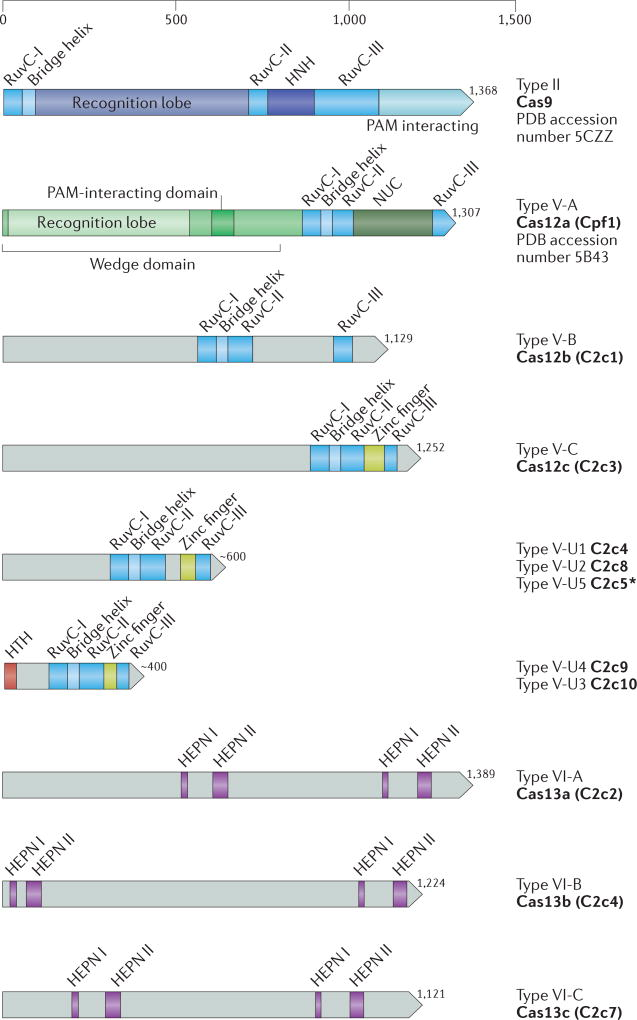
\includegraphics[scale=1]{nihms945745f2}
\label{fig:nihms945745f2}
\caption {A arquitetura de domínio das proteínas efetoras \ac{crispr} de classe 2}
\end{figure}



\chapter{Anti-CRISPRs}
\label{chap.anti-CRISPRs}

Por sua vez em resposta os fagos são frequentemente codificados inibidores do sistema imunológico bacteriano que aumentam sua capacidade de "lisar" (realizar lise celular) a bactéria hospedeira ou de se integrar ao seu genoma (Samson et al., 2013). Os primeiros exemplos de proteínas "anti-CRISPR" codificadas por fago vieram para os sistemas de classe 1 tipo I-F e I-E em Pseudomonas aeruginosa (Bondy-Denomy et al., 2013, Pawluk et al., 2014). Notavelmente, dez genes anti-CRISPR tipo IF e quatro genes anti-CRISPR tipo IE foram descobertos até o momento (Pawluk et al., 2016), todos os quais codificam proteínas pequenas e distintas (50-150 aminoácidos), anteriormente de função desconhecida . Nossa investigação bioquímica de quatro proteínas I-F anti-CRISPR revelou que elas interagem diretamente com diferentes proteínas Cas no complexo multiproteína \ac{crispr}-Cas para prevenir o reconhecimento ou clivagem do DNA alvo (Bondy-Denomy et al., 2015). As proteínas anti-CRISPR têm sequências distintas (Bondy-Denomy et al., 2013), estruturas (Maxwell et al., 2016, Wang et al., 2016) e modos de ação (Bondy-Denomy et al., 2015). Essas descobertas apóiam a evolução independente dos inibidores \ac{crispr}-Cas e sugerem que muitos mais ainda estão para ser descobertos. De fato, uma investigação recente explorou a conservação da assinatura do gene associado a anti-CRISPR (aca) com um motivo de hélice-volta-hélice (HTH) previsto para identificar anti-CRISPRs em proteobactérias, abrangendo amplamente a filogenia do tipo IF \ac{crispr}-Cas (Pawluk et al., 2016).\par

Atualmente não se sabe se as proteínas anti-CRISPR ocorrem em outros filos bacterianos, apesar dos anti-CRISPRs serem comuns e diversos dentro das proteobactérias. Da mesma forma, também não está claro se existem anti-CRISPRs para sistemas diferentes dos tipos I-E e I-F. Em P. aeruginosa, os anti-CRISPRs tipo I são expressos a partir de genomas de fagos integrados (profagos) e causam a inativação constitutiva do sistema \ac{crispr}-Cas hospedeiro (Bondy-Denomy et al., 2013). Nesses casos, o profago pode possuir um alvo de DNA com perfeita identidade a um espaçador \ac{crispr} na mesma célula, pois o sistema \ac{crispr}-Cas está inativado. A coocorrência genômica de um espaçador e seu DNA-alvo com uma correspondência perfeita é chamada de "auto-direcionamento" (Figura 1A). Bactérias com auto-direcionamento requerem inativação de \ac{crispr}-Cas para sobrevivência; na ausência de genes anti-CRISPR, o genoma do hospedeiro será clivado no ato de direcionar o profago (Bondy-Denomy et al., 2013, Edgar e Qimron, 2010). A expressão de um anti-CRISPR neutraliza esse risco. Supomos que os genomas que possuem um sistema \ac{crispr} com aparente auto-direcionamento seriam candidatos para a identificação de novos inibidores \ac{crispr}-Cas. Aqui, nós descrevemos a identificação de quatro inibidores \ac{crispr}-Cas9 codificados por fago anteriormente desconhecidos em Listeria monocytogenes usando uma abordagem de bioinformática para identificar incidentes de auto-direcionamento. Também demonstramos que dois desses inibidores podem bloquear a atividade de S. pyogenes Cas9 em células bacterianas e humanas.


\begin{figure}[h]
\center
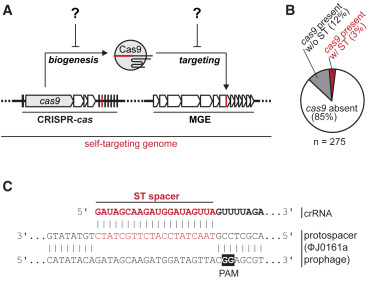
\includegraphics[scale=1]{gop}
\label{gop}
\caption {Uma pesquisa para \ac{crispr}-Cas9 Genomic Self-Targeting em Listeria monocytogenes (A) Um esquema que descreve o princípio de auto-direcionamento genômico, em que um elemento genético móvel (MGE) possui uma sequência alvo para um espaçador em uma matriz \ac{crispr} no mesmo genoma. A função \ac{crispr}-Cas9 neste "genoma de auto-direcionamento" é presumivelmente inativa para a viabilidade celular contínua.
(B) A abundância de genomas com (vermelho) e sem (cinza) auto-direcionamento ligado a cas9 (ST), em genomas de L. monocytogenes. Consulte a Tabela S1 para uma lista de cepas de auto-direcionamento.
(C) Um exemplo de um evento ST, onde o espaçador 16 no arranjo \ac{crispr} tipo II-A da cepa J0161 tem uma correspondência perfeita de PAM e protoespaçador com um profago residente .}
\end{figure}


\chapter{Aplicação}
\label{chap.aplicação}

O \ac{crispr} já apresentou resultados promissores no tratamento de diversas doenças e também teve um grande impacto na edição de genomas de plantas, facilitando diversas aplicações agrícolas benéficas. A tecnologia \ac{crispr} também mostrou potencial em outras áreas, como o desenvolvimento de modelos de doenças e biocombustíveis. 

\section{Eliminar doenças}

No ano passado, o bioengenheiro Daniel Anderson do Massachusetts Institute of Technology em Cambridge e seus colegas usaram o \ac{crispr} em camundongos para corrigir uma mutação associada a uma doença metabólica humana chamada tirosinemia5. Foi o primeiro uso do \ac{crispr} para corrigir uma mutação causadora de doença em um animal adulto - e um passo importante no sentido de usar a tecnologia para terapia genética em humanos (ver ‘Uma breve história do \ac{crispr}’).

A ideia de que o \ac{crispr} poderia acelerar o campo da terapia genética é uma grande fonte de entusiasmo nos círculos científicos e de biotecnologia. Mas, além de destacar o potencial, o estudo de Anderson mostrou o quanto ainda há a fazer. Para entregar a enzima Cas9 e seu RNA guia no órgão alvo, o fígado, a equipe teve que bombear grandes volumes de líquido para os vasos sanguíneos - algo que geralmente não é considerado viável em pessoas. E os experimentos corrigiram a mutação causadora da doença em apenas 0,4\% das células, o que não é suficiente para impactar muitas doenças.

Nos últimos dois anos, um punhado de empresas surgiu para desenvolver a terapia genética baseada no \ac{crispr}, e Anderson e outros dizem que os primeiros testes clínicos desse tipo de tratamento poderiam acontecer nos próximos um ou dois anos. Esses primeiros testes provavelmente serão cenários nos quais os componentes do \ac{crispr} podem ser injetados diretamente nos tecidos, como os do olho, ou nos quais as células podem ser removidas do corpo, projetadas no laboratório e depois colocadas de volta. Por exemplo, as células-tronco formadoras de sangue podem ser corrigidas para tratar doenças como a doença das células falciformes ou Beta-talassemia. 
Um maior desafio será entregar a enzima e direcionar o RNA em vários outros tecidos, os pesquisadores, no entanto, esperam que a técnica possa um dia ser usada para combater
 uma gama mais ampla de doenças genéticas.

\section{Na alimentação}
Enquanto Anderson e outros têm como objetivo modificar o DNA em células humanas, outros estão visando plantações e gado. Antes da chegada das técnicas de edição de genes, isso geralmente era feito pela inserção de um gene no genoma em posições aleatórias, junto com sequências de bactérias, vírus ou outras espécies que conduzem a expressão do gene. Mas o processo é ineficiente e sempre foi alimento para críticos que não gostam da mistura de DNA de espécies diferentes ou temem que a inserção possa interromper outros genes. Além disso, obter a aprovação de safras geneticamente modificadas para uso é tão complexo e caro que a maioria das que foram modificadas são grandes safras de commodities, como milho (milho) e soja.

\begin{figure}[h]
\center
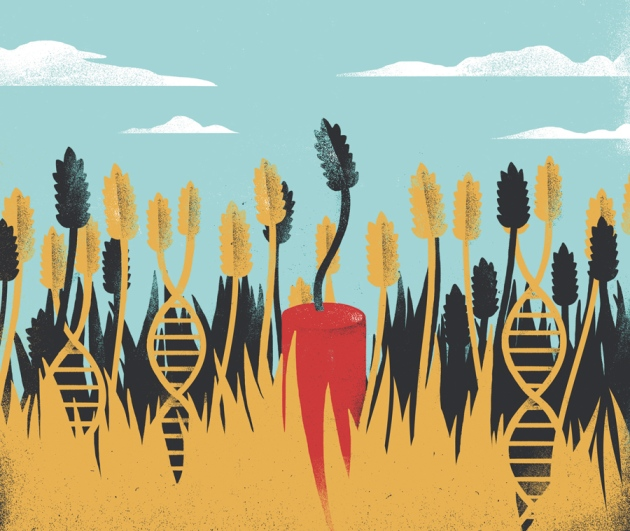
\includegraphics[scale=0.4]{farm}
\label{farm}
\caption {Ilustração de plantas geneticamente alteradas por Sébastien Thibault}
\end{figure}

Com o \ac{crispr}, a situação pode mudar: a facilidade e o baixo custo podem tornar a edição do genoma uma opção viável para culturas menores e especiais, bem como para animais. Nos últimos anos, os pesquisadores usaram o método para projetar porcos pequenos e para fazer trigo e arroz resistentes a doenças. Eles também fizeram progressos na engenharia de gado descornado, cabras resistentes a doenças e laranjas doces enriquecidas com vitaminas. Doudna antecipa que sua lista de organismos modificados pelo \ac{crispr} aumentará. “Há uma oportunidade interessante de considerar a realização de experimentos ou caminhos de engenharia em plantas que não são tão importantes comercialmente, mas são muito interessantes do ponto de vista da pesquisa - ou para hortas caseiras”, diz ela.

A capacidade do \ac{crispr} de editar com precisão as sequências de DNA existentes torna as modificações mais precisas, mas também torna mais difícil para os reguladores e fazendeiros identificar um organismo modificado uma vez que tenha sido liberado. “Com a edição de genes, não há mais a capacidade de rastrear produtos de engenharia”, diz Jennifer Kuzma, que estuda política científica na North Carolina State University em Raleigh. “Será difícil detectar se algo sofreu uma mutação convencional ou geneticamente modificada”.

Isso soa o alarme para os oponentes das safras geneticamente modificadas e coloca questões difíceis para os países que estão tentando descobrir como regular plantas e animais editados por genes. Nos Estados Unidos, a Food and Drug Administration ainda não aprovou qualquer animal geneticamente modificado para consumo humano e ainda não anunciou como tratará os animais com edição genética.

De acordo com as regras existentes, nem todas as safras feitas por edição de genoma exigiriam regulamentação do Departamento de Agricultura dos Estados Unidos (ver Nature 500, 389-390; 2013). Mas, em maio, o departamento de agricultura começou a buscar sugestões sobre como melhorar a regulamentação de plantações geneticamente modificadas - uma medida que muitos interpretaram como um sinal de que a agência está reavaliando suas regras à luz de tecnologias como o \ac{crispr}. “A janela foi quebrada”, diz Kuzma. “O que passa pela janela fica para ver. Mas o fato de que ele foi quebrado é muito emocionante. ”

\section{Ecossistemas projetados}


Além de quintas, os pesquisadores estão considerando como o \ac{crispr} pode ou deve ser implantado em organismos na natureza. Grande parte da atenção se concentrou em um método chamado gene drive, que pode varrer rapidamente um gene editado por uma população. O trabalho está em um estágio inicial, mas essa técnica poderia ser usada para exterminar mosquitos ou carrapatos transmissores de doenças, eliminar plantas invasoras ou erradicar a resistência a herbicidas em pigweed, que assola alguns agricultores dos EUA.

Normalmente, uma mudança genética em um organismo leva muito tempo para se espalhar por uma população. Isso ocorre porque uma mutação carregada em um dos dois cromossomos é herdada por apenas metade da prole. Mas uma unidade genética permite que uma mutação feita por \ac{crispr} em um cromossomo se copie para seu parceiro em cada geração, de modo que quase todos os descendentes herdarão a mudança. Isso significa que ele irá acelerar através de uma população exponencialmente mais rápido do que o normal (veja 'Gene drive') - uma mutação projetada em um mosquito pode se espalhar por uma grande população em uma temporada. Se essa mutação reduzisse o número de descendentes produzidos por um mosquito, a população poderia ser exterminada, junto com quaisquer parasitas da malária que carregue.


Publicações: Scopus; Patentes: The Lens; Financiamento: NIH RePORTER.

\begin{figure}[h]
\center
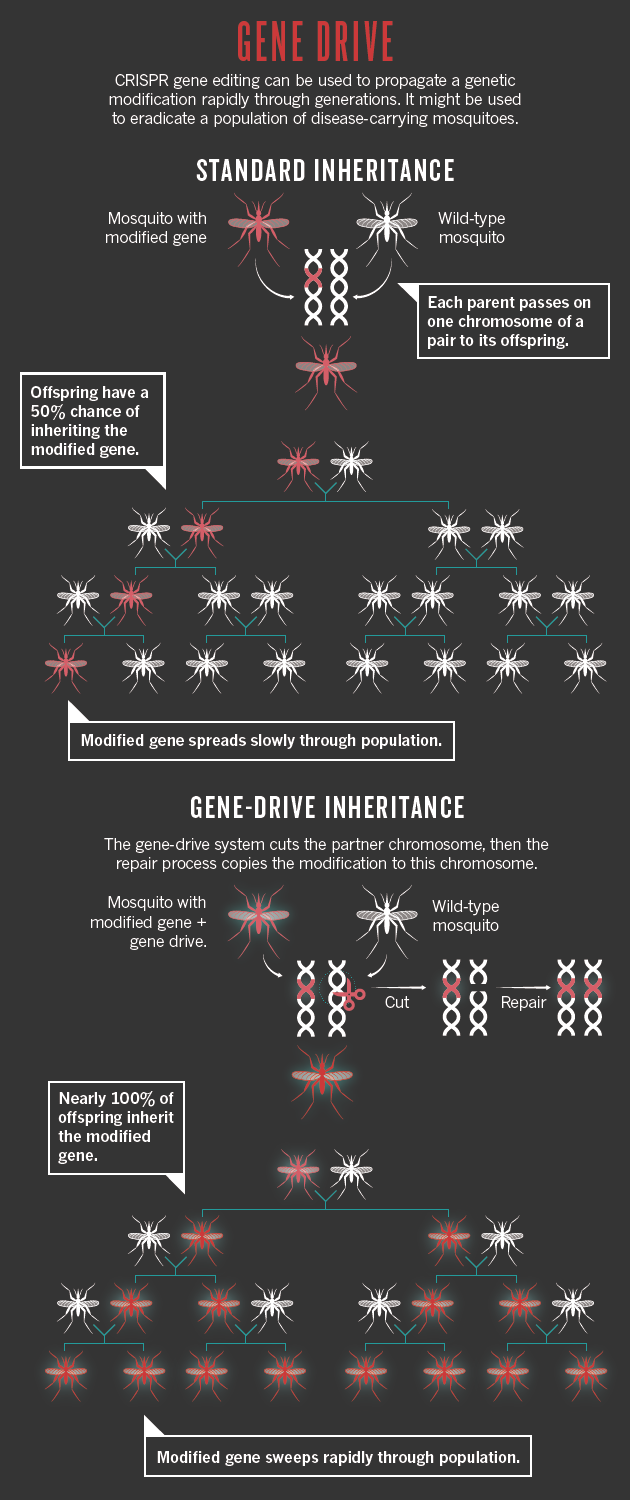
\includegraphics[scale=0.4]{lmao}
\label{lmao}
\caption {Publications: Scopus; Patents: The Lens; Funding: NIH RePORTER.}
\end{figure}




Mas muitos pesquisadores estão profundamente preocupados com o fato de que alterar uma população inteira, ou eliminá-la por completo, pode ter consequências drásticas e desconhecidas para um ecossistema: pode significar que outras pragas surgem, por exemplo, ou pode afetar predadores em níveis superiores na cadeia alimentar. E os pesquisadores também estão cientes de que um RNA-guia pode sofrer mutações com o tempo, de modo a atingir uma parte diferente do genoma. Essa mutação poderia então se espalhar pela população, com efeitos imprevisíveis.

“Tem que ter um retorno bastante alto, porque tem um risco de irreversibilidade - e consequências indesejadas ou difíceis de calcular para outras espécies”, diz George Church, bioengenheiro da Harvard Medical School em Boston. Em abril de 2014, Church e uma equipe de cientistas e especialistas em políticas escreveram um comentário na Science6 alertando os pesquisadores sobre os riscos e propondo formas de proteção contra a liberação acidental de unidades genéticas experimentais.

Na época, os impulsos genéticos pareciam uma perspectiva distante. Porém, menos de um ano depois, o biólogo do desenvolvimento Ethan Bier, da Universidade da Califórnia, em San Diego, e seu aluno Valentino Gantz relataram que haviam projetado esse sistema em moscas-das-frutas7. Bier e Gantz usaram três camadas de caixas para conter suas moscas e adotaram medidas de segurança de laboratório geralmente usadas para mosquitos transmissores da malária. Mas eles não seguiram todas as diretrizes sugeridas pelos autores do comentário, como conceber um método para reverter a mudança projetada. Bier diz que eles estavam conduzindo seus primeiros experimentos de prova de princípio e queriam saber se o sistema funcionava antes de torná-lo mais complexo.

Para Church e outros, esse foi um aviso claro de que a democratização da edição do genoma por meio do \ac{crispr} poderia ter resultados inesperados e indesejáveis. “É essencial que as autoridades regulatórias nacionais e as organizações internacionais tomem conta disso - realmente tomem conta disso”, diz Kenneth Oye, cientista político do Instituto de Tecnologia de Massachusetts e principal autor do comentário Science. “Precisamos de mais ação.” O Conselho Nacional de Pesquisa dos Estados Unidos formou um painel para discutir os impulsos genéticos e outras discussões de alto nível estão começando a ocorrer. Mas Oye está preocupado com o fato de que a ciência está avançando na velocidade da luz e que as mudanças regulatórias podem acontecer apenas após uma liberação de gene impulsionada de alto perfil.





O problema não é preto e branco. Micky Eubanks, ecologista de insetos da Texas A\&M University em College Station, diz que a ideia dos impulsos genéticos o chocou no início. “A minha reação inicial foi 'Meu Deus, isso é terrível. É tão assustador '”, diz ele. “Mas quando você pensa mais e pesa em relação às mudanças ambientais que já fizemos e continuamos a fazer, seria uma gota no oceano.”

Alguns pesquisadores vêem lições para o \ac{crispr} no arco de outras novas tecnologias que geraram grande empolgação, preocupação e decepção quando surgiram problemas iniciais. O geneticista médico James Wilson, da Universidade da Pensilvânia, na Filadélfia, estava no centro do entusiasmo crescente pela terapia genética na década de 1990 - apenas para testemunhar sua queda quando um ensaio clínico deu errado e matou um jovem. O campo entrou em parafuso e só recentemente começou a se recuperar. O campo \ac{crispr} ainda é jovem, diz Wilson, e pode levar anos até que seu potencial seja realizado. “Está em fase de exploração. Essas ideias precisam fermentar. ”\par

Então, novamente, Wilson foi mordido pelo bug \ac{crispr}. Ele diz que era cético em relação a todas as promessas feitas a respeito até que seu próprio laboratório começou a brincar com a técnica. “Em última análise, terá um papel na terapêutica humana”, diz ele. “É realmente espetacular.”





\chapter{Conclusões}
\label{chap.conclusões}
Uma importante questão ética em pesquisa é que os benefícios devem superar os riscos.
É proposto por parte de especialistas que se dê mais atenção aos riscos, visto que o seu impacto em seres vivos ou no ambiente pode ser extremamente prejudicial. 

Desta forma governos e instituições devem responder, com o intuito de evitar esses perigos, estabelecendo padrões com o intuito de permitir pesquisas promissoras avançarem e garantindo à população que o trabalho está sendo conduzido responsavelmente.




\chapter*{Contribuições dos autores}

Este projeto foi realizado na totalidade por mim, Alexandre Martins, 103552.

%%%%%%%%%%%%%%%%%%%%%%%%%%%%%%%%%
\chapter*{Acrónimos}
\begin{acronym}
\acro{ua}[UA]{Universidade de Aveiro}
\acro{miect}[MIECT]{Mestrado Integrado em Engenharia de Computadores e Telemática}
\acro{glisc}[GLISC]{Grey Literature International Steering Committee}
\acro{crispr}[CRISPR]{Clusters of regularly interspaced short palindromic repeats}



\end{acronym}


%%%%%%%%%%%%%%%%%%%%%%%%%%%%%%%%%
\chapter*{Bibliografia}
\begin{flushleft}

CRISPR, the disruptor, https://www.nature.com/news/crispr-the-disruptor-1.17673.\par




Inhibition of CRISPR-Cas9 with Bacteriophage Proteins, https://www.sciencedirect.com/science/article/pii/S009286741631683X.\par




CRISPR/Cas, https://pt.wikipedia.org/wiki/CRISPR/Cas.\par
CRISPR, https://pt.wikipedia.org/wiki/CRISPR.\par
Cas9, https://pt.wikipedia.org/wiki/Cas9.\par
Exploring class 1 CRISPR systems, https://www.nature.com/articles/s41592-019-0642-1.\par
Diversity and evolution of class 2 CRISPR–Cas systems, https://www.ncbi.nlm.nih.gov/pmc/articles/PMC5851899/.

\end{flushleft}


\printbibliography

\end{document}
